\documentclass{article}

\usepackage{hyperref}
\usepackage{float}
\usepackage{graphicx}
\usepackage{subcaption}
\usepackage{bookmark} % Added to handle rerunfilecheck warning

\title{Software Engineering\\ Rapport}
\author{Pierre Louis 23317}
\date{academic year 2024-2025}

\begin{document}

\maketitle

\section{Introduction}
This is our report of our project in software engineering.

\section{activity diagramme}

\begin{figure}[H]
    \centering
    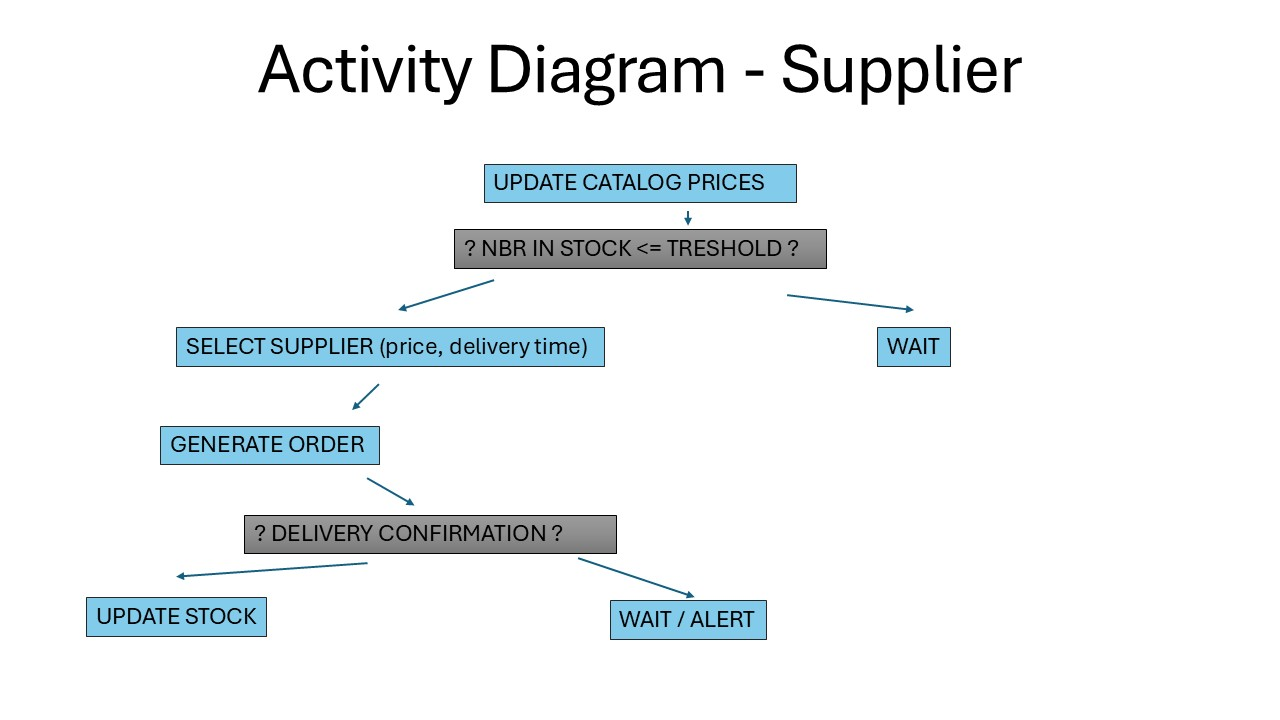
\includegraphics[width=0.8\textwidth]{images/activity_diagram1.JPG}
    \caption{first image}
    \label{fig:image1}
\end{figure}

\begin{figure}[H]
    \centering
    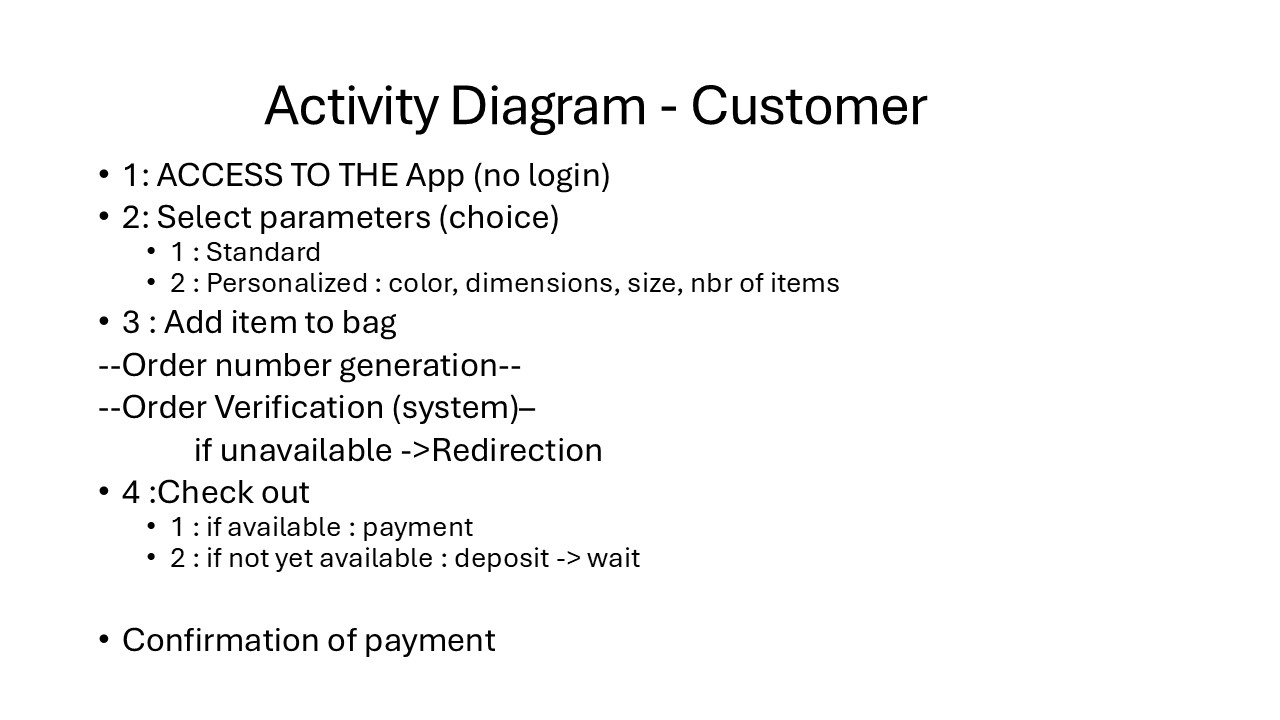
\includegraphics[width=0.8\textwidth]{images/activity_diagram2.JPG}
    \caption{second image}
    \label{fig:image2}
\end{figure}

\section{Use case diagramme}

\section{user state diagram}

\begin{figure}[H]
    \centering
    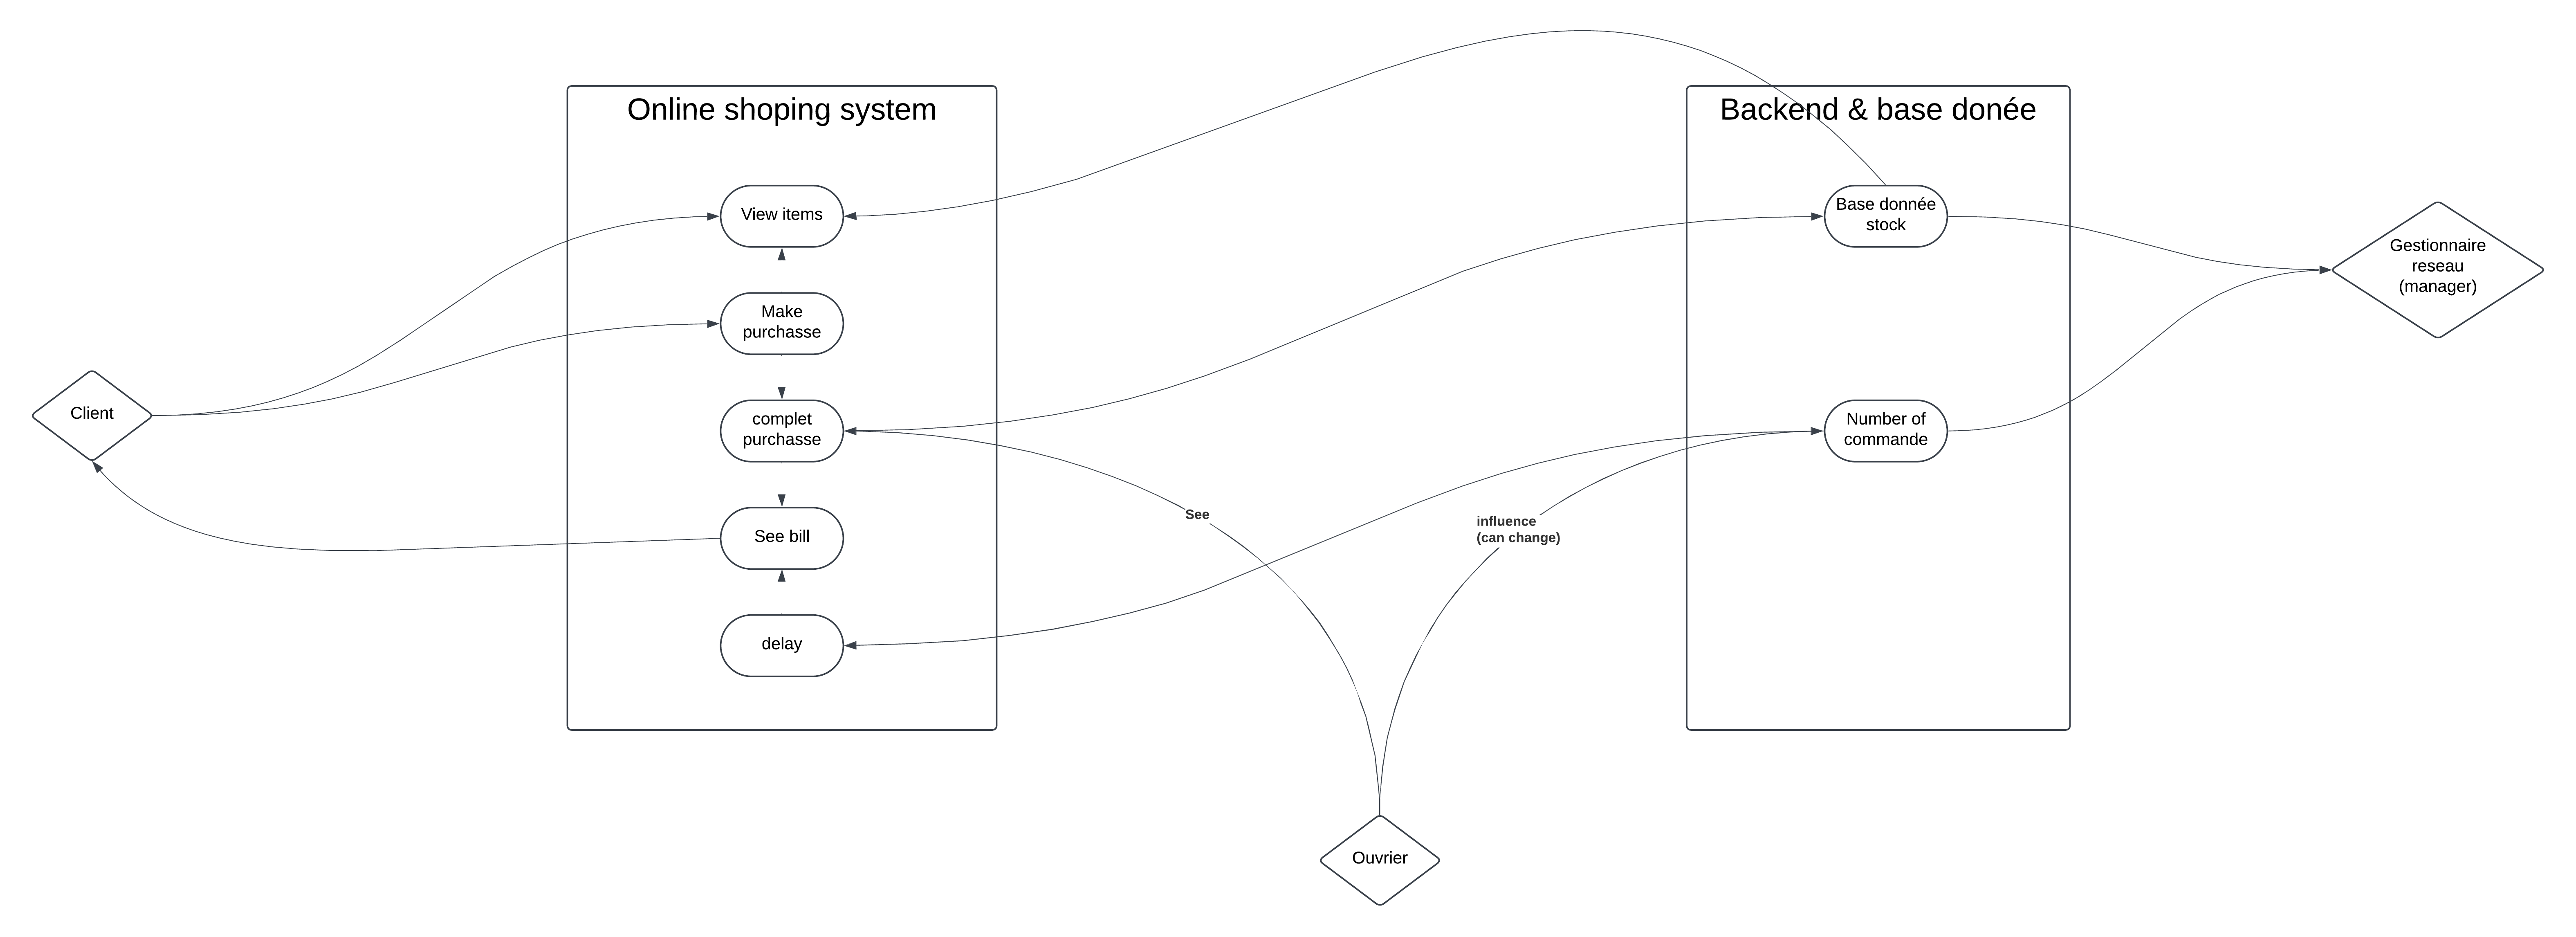
\includegraphics[width=0.8\textwidth]{images/user_state_diagram.png}
    \caption{User State Diagram}
    \label{fig:user_state_diagram}
\end{figure}

\section{User stories}

Here is a sample of user stories: we have made and the conclusion.

\paragraph{user story 1}:
As a customer, I want to configure a cabinet with customizable dimensions, colors, and
optional doors, so that I can place my order accurately and ensure compatibility of parts
before visiting the store.
\subparagraph{Acceptance criteria}:
\begin{itemize}
    \item design and configuration
    \begin{itemize}
        \item The customer can select the number of lockers (up to 7).
        \item The customer can specify the dimensions (height, width, depth) of each locker, based on catalog constraints.
        \item The customer can choose colors for panels, doors, and angle irons from the catalog.
        \item Compatibility rules (e.g., maximum door dimensions, height of angle irons) are validated automatically by the application.
    \end{itemize}
    \item order verification
    \begin{itemize}
        \item The system prevents incorrect configurations (e.g., incompatible parts).
        \item The application displays real-time availability of parts in stock.
        \item If parts are out of stock, the system prompts the user to pay a deposit and provides an estimated availability date
    \end{itemize}
    \item Invoice and Payment
    \begin{itemize}
        \item The application generates an invoice for the customer upon confirmation.
        \item Payment options include deposit for out-of-stock items and full payment on receipt of parts.
    \item Future-Proof Architecture:
    \begin{itemize}
        \item The system supports future additions of components (e.g., shelves, drawers) without modifying existing functionality
    \end{itemize}
    \end{itemize}

\end{itemize}

\section{Relationship entity diagram}

\section{Class diagram and sequence diagramme}

\section{User manual}

\section{Backend}

\section{Link}
\href{https://github.com/I42I/Kitbox_app}{Github Project}
\href{https://github.com/PierreLouis-23317/Software2_report/settings/access}{report LaTeX}


\section{Conclusion}

\end{document}